\documentclass{sig-alternate}

\usepackage{url} 
\usepackage{subfigure} 
\usepackage{color}
\usepackage{graphicx}
\usepackage{xspace}
\usepackage{listings}


\usepackage[font=footnotesize]{subfig}
\DeclareCaptionType{copyrightbox}
\hyphenation{op-tical net-works semi-conduc-tor}

\newif\ifdraft
\drafttrue
\ifdraft
\newcommand{\tbnote}[1]{ {\textcolor{magenta} { ***TcB: #1 }}}
\newcommand{\jhanote}[1]{ {\textcolor{red} { ***SJ: #1 }}}
\newcommand{\mrnote}[1]{ {\textcolor{blue} { ***Melissa: #1 }}}
\newcommand{\egnote}[1]{ {\textcolor{green} { ***Emilio: #1 }}}
\newcommand{\hfnote}[1]{ {\textcolor{cyan} { ***HF: #1 }}}
\newcommand{\rajib}[1]{ {\textcolor{blue} { ***RM: #1 }}}
\else
\newcommand{\rajib}[1]{}
\newcommand{\jhanote}[1]{}
%\newcommand{\note}[1]{ {\textcolor{blue} { ***NOTE: #1 }}}
\newcommand{\note}[1]{ {}}
\newcommand{\abhi}[1]{ {}}
\newcommand{\hfnote}[1]{}
\newcommand{\tbnote}[1]{ {}}
\fi

\newcommand{\pilotjob}{Pilot-Job\xspace}
\newcommand{\pilotjobs}{Pilot-Jobs\xspace}
\newcommand{\pilotdata}{Pilot-Data\xspace}
\newcommand{\pilotapi}{Pilot-API\xspace}

\begin{document}

\conferenceinfo{XSEDE13}{'13 }
 \CopyrightYear{2013}

 \title{A Framework for Flexible and Scalable Replica-Exchange on
   Production Distributed CI}

\numberofauthors{5} 
\author{
\alignauthor
Brian Raddak \\
       \affaddr{BioMaPS Institute for Quantitative Biology and Department of Chemistry and Chemical Biology, Rutgers University}\\
       \affaddr{Piscataway, NJ 08854}\\
       \affaddr{Department of Chemistry, University of Minnesota}\\
       \affaddr{Minneapolis, MN 55455}\\
      \email{x}
\alignauthor
Melissa Romanus\\
       \affaddr{Rutgers University}\\
       \affaddr{Piscataway, NJ 08854}\\
      \email{x}
\alignauthor
Emilio Gallichio\\
       \affaddr{Rutgers University}\\
       \affaddr{Piscataway, NJ 08854}\\
      \email{x}
\and  % use '\and' if you need 'another row' of author names
% 3rd. author
\alignauthor 
Taisung Lee \\
       \affaddr{BioMaPS Institute for Quantitative Biology and Department of Chemistry and Chemical Biology, Rutgers University}\\
       \affaddr{Piscataway, NJ 08854}\\
      \email{taisung@biomaps.rutgers.edu}
\alignauthor
Ole Weidner \\
       \affaddr{Rutgers University}\\
       \affaddr{Piscataway, NJ 08854}\\
      \email{xxx}
\alignauthor 
Darrin York \\
       \affaddr{BioMaPS Institute for Quantitative Biology and Department of Chemistry and Chemical Biology, Rutgers University}\\
       \affaddr{Rutgers University}\\
       \affaddr{Piscataway, NJ 08854}\\
      \email{york@biomaps.rutgers.edu}
\and
\alignauthor 
Ron Levy \\
       \affaddr{Rutgers University}\\
       \affaddr{Piscataway, NJ 08854}\\
       \email{xxx}
\alignauthor 
Shantenu Jha \\
       \affaddr{Rutgers University}\\
       \affaddr{Piscataway, NJ 08854}\\
       \email{xxx}
}

\maketitle

\begin{abstract}

  A description of the computational workflow, viz., the different
  machines/resources used, how many ensembles we simulated, data
  volumnes managed etc., (ii) any computational performance issues
  including (a) measuring "efficiency" as the number of distributed
  resources utilized goes as measured by $T_c$ (time to completion),
  (b) $T_c$ as a function of the number of replicas, and (iii) a
  description of the software infrastructure that is employed to
  enable distributed replica-exchange on XSEDE.
  \jhanote{SJ}
\end{abstract}

\category{H.4}{Information Systems Applications}{Miscellaneous}
%A category including the fourth, optional field follows...
\category{D.2.8}{Software Engineering}{Metrics}[complexity measures, performance measures]

\terms{Experience, Technology}

\keywords{HPC, Distributed Computing, IMPACT, AMBER, MD, Large Scale, XSEDE
  resources}

\section{Introduction}
\jhanote{SJ + Emilio Section}

Although the coupling between replicas is conceptually simple and
relatively ``easy'', replica-exchange applications represent the
general challenge of scaling many loosely-coupled simulations. The
challenge arises from the fact that although most communication is
internal to the individual replicas which are large-scale MPI-style
simulations, there exist a less frequent but often a slow
communication mode which increases in complexity, importance and cost
as the number of replicas increases. Providing an approach that works
across multiple replica sizes, replica numbers and coupling schemes
both a software and conceptual challenge.

To address some of these issues, there has been recent progress
towards a pilot-job based replica-exchange framework, that can support
dynamic and scalable resource execution and management, and thereby
provides the basis for a flexible and scalable formulation of
replica-exchange. ..


\jhanote{Describe the need for large-scale simulations. Describe what
  is unique to replica-exchange. Challenges that arise from loose,
  intermittent (stochastic) coupling, as opposed to fixed exchanges}

Parallel Replica Exchange (RE) denotes a family of advanced
conformational sampling algorithms widely employed in molecular
simulations of chemical and biological systems. The key aspect of RE
algorithms is that multiple molecular dynamics (MD) threads (referred
to as “replicas”) each assigned to a different thermodynamic or
potential energy state of the system, are executed in parallel and, further,
replicas travel in configurational space as well as in state
space by communicating and stochastically exchanging their state
assignments with those of other replicas. Exchanges are controlled by
microscopic reversibility requirements ensuring that feasible
thermodynamic ensembles are sampled at each state.  It has been shown
in many contexts \egnote{[references]} that RE moves enhance
conformational mixing relative to multiplexed serial conformational
sampling algorithms based on teams of non-communicating
MD threads. Replica exchange algorithms indeed provide some of the
most powerful conformational sampling tools available, yielding
converged results orders of magnitude faster than
conventional approaches.

The advantages of RE approaches are however partly counterbalanced by
the additional complexities inherent in instating and maintaining a
communication framework among the MD threads. In practice this
requirement has historically discouraged large scale deployment of RE
on XSEDE. In our view this is not necessarily due to lack of suitable
hardware and networking resources, but rather to the lack of suitable
software technologies capable of efficiently harnessing this latent
computational power.

Many applications areas, such as the ones illustrated in this report,
benefit greatly from multi-dimensional RE implementations employing
hundreds to thousands of replicas. However, current implementations
of the replica exchange method in use by the computational chemistry
community are severely limited in terms of it scalability and control
when many replicas are involved. In conventional implementations of
RE, simulations progress in unison and exchanges occur in a
synchronous manner whereby all replicas must reach a pre-determined
state (typically the completion of a certain number of MD steps),
before exchanges are performed. This synchronous approach has a number
of severe limitations. Firstly, sufficient dedicated computational
resources must be secured for all of the replicas before the
simulation can begin execution. Secondly, the computational resources
must be statically maintained until the simulation is
completed. Thirdly, failure of any replica simulation typically causes
the whole calculation to abort. The reliance on a static pool of
computational resources and zero fault tolerance prevents the
synchronous RE approach from being a feasible solution for large scale
RE deployments.

As earlier prototypical implementations of asynchronous RE (aRE)
algorithms \egnote{[Gallicchio 2008]} have illustrated, the replica
exchange method itself does not impose the restriction that exchanges
should occur synchronously across all threads and that all of the MD
threads should run at the same time. The basic idea of asynchronous
RE is to allow pairs of replicas to perform exchanges independently
from the other replicas. This paradigm lends itself naturally to
implementations based on the pilot-job framework described below,
which, while already extensively employed to automate the asynchronous
execution of independent ensembles, as shown in this work, can be
effectively employed to manage inter-communicating MD threads.

In this work we present ASyncRE, an asynchronous RE software utility
deployed built on the BigJob/SAGA distributed computing environment on
XSEDE capable of scaling to arbitrarily large numbers of
replicas. Illustrative applications of the software to large-scale
multi-dimensional RE problems are presented and analyzed ...

\jhanote{(i) algorithmic advances coupled with infrastructural
  advances. (ii) the need for dynamic execution and resource
  management, (iii) which is why we believe pilot-jobs is a good
  abstraction (reference earlier work using BigJob). (iv) Novelty of
  this work is: (A) marriage of an application library for flexible
  replica-exchange simulations with scalable and dynamic resource
  management, (B) demonstration of a framework for different and
  tunable replica coupling schemes that can be used for QM and
  classical examples.}
 
\jhanote{Aim of this work is to present (i) the framework -- both
  components, (ii) understand and characterize basic performance}


\section{Scientific Problem}\label{sec:requirements}

\jhanote{RE represents the core coordination/communication pattern for
  a class of problems} 

The conformational sampling problem in molecular simulations can be
described as the problem of efficiently drawing samples $x$ from the
canonical distribution of the chemical system:
\begin{equation}
p(x;\beta,\theta) = \frac{\exp[-U(x;\beta,\theta)]}{Z} \, ,
\end{equation}
where $x$ represents the configuration of the system (atomic
coordinates), $Z$ denotes the configurational partition function,
$\beta=1/k_B T$ is the inverse temperature, and
$U(x;\beta,\theta)=\beta V(x;\theta)$ is the dimensionless potential
energy of the system which depends linearly on the set inverse temperature
(generally also on the applied pressure and the chemical potentials of
the components for the isobaric and grand-canonical ensembles,
respectively) and on potential energy parameters (such as partial
charges etc., as well as parameters of applied biasing potentials)
collectively denotes as $\theta$.

In conventional MD-based conformational sampling implementations $x$
evolves in time while the parameters of the model ($\beta$ and
$\theta$) are kept fixed. Slow convergence is the main issue of
concern of methods of this kind as it is notoriously difficult to
achieve equilibration within the time scale afforded by even the
fastest supercomputers. Great progress has been achieved in recent
years with the development of generalized ensemble formulations which
provide a random walk not only in conformational space,
but also in parameter space.  Enhanced conformational sampling
algorithms based on generalized ensembles have revolutionized the
field allowing the modeling of complex biochemical processes with
unprecedented fidelity.

Amongst generalized ensemble conformational sampling algorithms, replica exchange (RE)
algorithms (introduced above) are some of the most effective and, in addition,
particularly suitable for deployment on parallel computing architectures. RE is based on
teams of MD threads each traveling in state space by exchanging state parameters
($\beta_i$,$\theta_i$) among each other.  The most widely employed RE scheme is
temperature RE (T-RE) in which inverse temperatures $\beta_i$ are exchanged. T-RE
accelerates interconversions between stable states of the system by letting replicas
temporarily visit high temperatures where barrier crossings are facilitated. However, RE
schemes can involve exchanges of any number of state parameters. RE schemes involving
the exchange of more than one parameters are often referred to as
\emph{multi-dimensional} RE schemes.

Any RE scheme is required to satisfy microscopic reversibility. In the present context
this is ensured by structuring RE exchanges so that permutations of state parameters
assignments to replicas are distributed according to the discrete unnormalized
probability distribution:
\begin{equation}
p(\{j_M\})=\exp\left[-\sum_{i=1}^M U(x_i;\beta_{j_i};\theta_{j_i}\right] \,
\end{equation}
where $\{j_M\}$ denotes one of the $M!$ permutations of an index vector of length $M$,  $x_i$ is the atomic configuration of replica $i$, and $\beta_{j_i}$ and $\theta_{j_i}$ are the inverse temperature and potential parameters sets assigned to replica $i$.

In this work we analyze four science application areas that benefit from the application of multi-dimensional RE protocols. The first is the modeling of binding between a guest molecule (cyclooctanol) and a host ($\beta$-cyclodextrin) to form a supramolecular complex in solution (Fig.\ \ref{}). In this case the dimensionless energy is:
\begin{equation}
U(x;\beta,\lambda) = \beta V_0(x) + \beta \lambda u(x) \,
\end{equation}
where $V_0(x)$ is the potential energy when the host and the guest are separated, $u(x)$ is the interaction energy between the host and the guest, and $\lambda$ is an alchemical parameter ranging between 0 and 1. This systems is modeled by multi-dimensional RE with up to 192 \egnote{modify as needed} replicas corresponding to all possible combinations of 8 temperatures distributed between 300 and 600K and 24 $\lambda$'s ranging between 0 and 1. The purpose of the sampling along $\lambda$ is to enhance mixing of conformations along the alchemical pathway while high temperatures enhance sampling at each alchemical stage.

The second application studied by multi-dimensional RE is the folding of the TrpCage mini-protein. In this case the dimensionless potential energy function is
\begin{equation}
U(x;\beta,\lambda) = \beta V(x) + \beta w_{\rm Go} V_{\rm Go}(x) \,
\end{equation}
where $V(x)$ is the unbiased potential energy, $V_{\rm Go}$ is a biasing potential favoring the formation of natively folded conformations, and $w_{\rm Go}$ is an energy weight ranging between 0 (no bias) to $0.42$ in this case (maximal bias). This system is studied with up to 336 \egnote{modify as needed} replicas corresponding to all possible combinations of 24 temperatures between 300 and 600K and 14 values of  $w_{\rm Go}$ between 0 and $0.42$. The purpose of this protocol is to bias the system so as to enhance the rate of folding and unfolding at multiple temperatures.

The last two applications employ multi-dimensional RE umbrella sampling (US), but in two
quite different scenarios, thus demonstrating the broad applicability of the approach.
In all multi-dimensional RE umbrella sampling simulations, the dimensionless potential
energy can be written as
\begin{equation}
U(x;\beta,\lambda) = \beta V_0(x) + \beta \sum_{n=1}^N W_n(x_n)
\end{equation}
where $V_0(x)$ is the unbiased potential and $W_n(x_n)$ is a bias potential applied to
the $n$th bias coordinate in order to localize sampling to high energy regions of
configuration space that might not otherwise be sampled. For convenience (as is
typically done) we choose $W_n(x_n)$ to have a harmonic form.  

In the first RE-US scheme, the well-known alanine dipeptide model for protein the
backbone is examined, and conformational biases are applied to the $\psi$/$\phi$ torsion
angles. The complete range of 360 degrees is divided into 15 degree intervals for both
angles, resulting in 576 replicas. Although this is a common test case for enhanced
sampling protocols
% Uncomment these citations if desired (see MDreferences.bib)
%%\cite{Chodera_JChemTheoryComput_2007_v3_p26,Chodera_JChemPhys_2011_v135_p194110}
, we increase the demand here by treating the solvent bath explicitly. The second
application is a phosphoryl transfer reaction in solution, a prototype reaction for
multiple protein and ribonucleic acid enzymes. Biases are applied to the breaking and
forming bonds. The chemically reactive solute is treated quantum mechanically, whereas
the solute is treated by classical molecular mechanics. 

Due to numerous calculations needed in quantum calculations and the unfavorable scaling
of these calculations (unlike classical force fields, quantum potentials cannot be
described as pair-wise interactions), it is extremely difficult to sample over the
conformational space to obtain sufficient and meaningful ensembles.  Hence the
advantages of a RE approach are especially important in QM simulations, such as the
example system present here.  The RE umbrella sampling is one of the most promising ways
to increase the feasible application of quantum potentials via increased sampling
efficiency.

\subsection{Describing the Replica-Exchange ``Workflow'' } \label{}

%\subsection{Computational Requirements}

\section{Software Environment}

XSEDE is inherently a complex infrastructure with heterogeneous
resources. In order to harness the power of such a distributed
environment, we utilize Pilot-Jobs. A Pilot-Job is a mechanism by 
which a proxy for the actual simulations
is submitted on the resource to be utilized; this proxy agent in turn,
is given responsibility to convey to the application the availabilty
of resources and also influence which tasks are executed. The
abstraction of a Pilot-Job generalizes the reoccurring concept of
utilizing a placeholder job as a container for a set of compute tasks;
instances of that placeholder job are commonly referred to as
Pilot-Jobs or pilots. 

In general, Pilot-Abstractions provide a suitable means to marshal
heterogeneous sets of both compute and data resources and support the
efficient utilization of different kinds of commercial as well science
cloud resources. Pilot-Abstractions have been extensively used on both
HPC and HTC infrastructures for a range of application scenarios as a
resource management abstraction to, (i) improve the utilization of
resources, (ii) to reduce wait times of a collection of tasks, (iii)
to facilitate bulk or high-throughput simulations where multiple jobs
need to be submitted which would otherwise saturate the queuing
system, and (iv) as a basis to implement application specific
execution, scheduling and policy decisions

The P* model~\cite{pstar12}, a model for Pilot-Abstractions, worked to
clearly define the computation and data components of a distributed
application as 'compute units' and 'data units' in the context of
Pilot-Jobs and Pilot-Data. A compute unit describes a self-containing
piece of work, e.g. a computational task that potentially operates on
a set of input data, while a data unit is a container for a logical
group of data that is often accessed together or comprises a larger
set of data; e.g. a data file or chunk.


\subsection{BigJob: A Pilot-based Framework}

%A specific implementation of the P* model is 
BigJob is a pilot-job system implementation which provides a framework
for running many types of distributed applications -- including but
not limited to very-large scale parallel simulations, many small
high-throughput simulations, or ensemble-based workflows. Consistent
with the P* model, BigJob (BJ) provides a unified runtime
environment for Pilot-Jobs on heterogeneous
infrastructures. For this purpose, BigJob provides a higher-level,
unifying interface to heterogeneous and/or distributed data and
compute resources. The framework is accessed via the Pilot-API, which
provides two key abstractions: Pilot-Job and Pilot-Data.

Applications can specify their resource requirements using a Pilot
description. In the compute case, the user typically specifies the
application to run as well as the number of cores required by their
application.  Pilots are started via the Pilot-Compute Service. BigJob 
eliminates the need to interact with different kinds of compute
resources, e. g. batch-style HPC/HTC resources as well as cloud
resources, and provides a unified abstraction for allocating
resources. 

BigJob has seen its widest usage across the heterogeneous resources
that XSEDE provides. Simple installation into user space on any
resource that supports Python 2.5 or greater makes the uptake of
BigJob easy for the end user. BigJob supports thousand of jobs and
millions of SUs on XSEDE and has been at the heart of two recent and
successful ECSS projects.

% BigJob has historically been used for parameter sweeps, many instances
% of the same task (ensemble), chained tasks, loosely coupled but
% distinct tasks, as well as tasks with data or compute dependencies.

\subsection{SAGA: Interoperability Layer}

In order for BigJob to work on heterogeneous resources, it requires an
interoperability layer which provides access to a variety of
middleware.  This is acheived through the use of The Simple API for Grid Applications (SAGA).
SAGA defines a 
high-level access mechanism for distributed infrastructure components 
like job schedulers, file transfers, and resource provisioning services. 
Given the heterogeneity of distributed infrastructures, SAGA provides 
a much needed interoperability layer that lowers the complexity and 
improves the simplicity of using distributed infrastructure whilst 
enhancing the sustainability of distributed applications, services, and tools.

SAGA is an Open Grid Forum (OGF) recognized standard (GFD.90). 
It allows developers of distributed applications to construct
higher-level functionality and abstractions, such as
gateways, workflows, application management systems, and runtime
environments. The key advantages to running with SAGA on XSEDE
is that users do not need to worry about the individual batch
queueing systems implemented on the various machines. Using the 
SAGA API and appropriate job adaptors, the different submission
mechanisms for these queueing systems is handled on the SAGA backend,
which is transpart to the user.

The SAGA API has been used to provide almost complete
coverage over nearly all grid and distributed computing
middleware/systems, including but not limited to Condor, Genesis,
Globus, UNICORE, SGE, LSF/PBS/Torque, and Amazon EC2.

\subsection{Using BigJob on XSEDE}

SAGA and BigJob are lightweight that they can be easily installed into
the home directory of a user using the Python Package Index
(PyPi). SAGA is packaged within BigJob, so users do not have to worry
about installing two seperate modules.

Since the main deployment is on XSEDE, we do not recommend altering
the default PYTHONPATH of the machines. Instead, we encourage users to
use a virtual environment. A virtual environment allows a user to
create a local Python software repository in his or her home directory
that behaves exactly like the global Python repository, except that it
grants the user \textit{write} access to it. In order to use virtual
environment, the Python version must be greater than 2.4. Since some
XSEDE machines use Python 2.4 as the default python version, it may be
required to load a python module file before installing BigJob.

After activating the virtual environment, the BigJob python package
can be installed by typing:

\begin{lstlisting}[frame=single]
easy_install bigjob
\end{lstlisting}

In addition to the BigJob package, it installs BigJob python
dependencies, including the SAGA package. The SAGA package includes
the proper adaptors for a wide variety of middleware systems. This
allows the user to submit jobs to almost any of the XSEDE batch
queuing systems.

BigJob requires SSH password-less login to the machines and a redis
server running either locally or on a remote server. The redis server
is used for coordination of the pilot-job and its compute and data
units. For the purposes of this project, we utilize a private redis
server hosted on a virtual machine at Indiana University. In order to
provide a more seemless uptake of BigJob by users, we will provide an
open-acess redis server available on XSEDE. This avoids the overhead
of new users having to start a redis-server on an XSEDE machine's head
node or on their local machines. This effort is currently underway
with XSEDE ECSS staff to make the server only accessible to registered
users of XSEDE.

After following the aforementioned steps, users will be able to write
their own BigJob submission scripts using Python. These scripts can
range from simple ensemble-based simulations to more complicated
workflows based on the users' needs.

\subsection{Async Replica-Exchange}
\mrnote{CompSci + PhysSci}

ASyncRE is a Python package to perform file-based asynchronous
parallel replica exchange molecular simulations. The current
implementation is aimed at computer clusters managed by a queuing
system and supported by a shared filesystem. The BigJob distributed
computing infrastructure is used for job launching and monitoring.

The ASyncRE package includes a core module which performs common tasks
such as job staging through BigJob and exchanging of parameters among
replicas. Support for arbitrary MD engines and RE schemes are
introduced through user-provided modules (Figure \ref{fig:aRE_chart}). Currently, MD
engine modules are available for the AMBER and IMPACT MD programs. A
similar modular mechanism provides support for arbitrary RE schemes
(temperature, Hamiltonian, etc.), including arbitrary multidimensional
combinations of these (such as 2D RE temperature/Hamiltonian). The
software is currently distributed with modules for multi-dimensional RE
umbrella sampling with AMBER\cite{AMBER12}, and BEDAM $\lambda$-RE alchemical binding
free energy calculations with the IMPACT MD engine \egnote{[BEDAM papers]}.

\begin{figure}
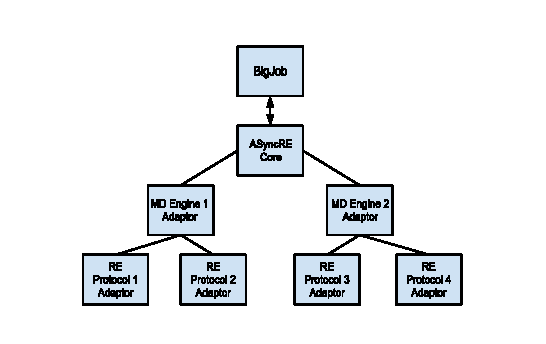
\includegraphics[width=3in]{asyncre.eps}
\caption{\label{fig:aRE_chart}The structure of the ASyncRE
  library. The ASyncRE Core module implements all of the
  general-purpose facilities to start and monitor replicas via BigJob,
  and coordinates replica exchanges. Routines implemented in adaptor
  modules perform functions specific to particular combinations of MD
  engines and RE schemes such as AMBER+umbrella sampling or IMPACT+BEDAM.  }
\end{figure}


The algorithm implemented by ASyncRE can be summarized as follows:

\begin{enumerate}

\item Job files and executables for the replicas are set up as
  appropriate for the MD engine/RE scheme combination as specified by
  the user-provided module/script. Typically this is accomplished by parsing a
  set of template input files according to the thermodynamic and
  potential energy settings which distinguish one replica from
  another. Each replica lives in a separate sub-directory of the
  working directory. These replica sub-directories are named
  \verb+r0+, {\tt r1}, $\ldots$,\verb+r<M-1>+, where \verb+M+ is the
  number of replicas.

\item Periodically, a randomly chosen subset of the replicas are
  submitted to BigJob for execution and enter a "R" (running)
  state. When a replica completes a run (of length specified in the MD
  engine input file), referred to in what follows as a "cycle", it
  enters a "W" (waiting) state which makes it eligible for exchange of
  thermodynamic and other parameters with other replicas and for the
  initiation of a new run cycle.

\item Periodically, exchanges of thermodynamic parameters are
  performed between the replicas in the waiting state based on the
  appropriate replica exchange rules (as specified in user modules)
  based on their thermodynamic states (temperature for example), or
  potential energy settings, together with the necessary structural
  and energetic information obtained from the MD engine output files.

\end{enumerate}

Internally a dictionary named \verb+status+ is used to keep track of
the status of the replicas (the current cycle, thermodynamic state,
running status, etc.) The status of the application is check-pointed
periodically using pickle. When restarting a previously stopped job,
the 'status' data structure is restored from this file and the
calculation proceeds from where it was left off.

An important feature of ASyncRE is the use of a ``run buffer'' to hide
latencies involved in the management of replica exchanges. Basically,
ASyncRE submits subjobs to BigJob in excess of the compute resources
allocated.  The result is that the submission of a replica
to BigJob for execution in general does not imply immediate execution;
rather, the replica is packaged in a BigJob compute unit which is
ready to begin execution as soon as BigJob can gather sufficient CPU
resources for it. In this way BigJob does not have to wait for a
replica to be prepared for a run cycle before it can execute it;
replicas are launched from a pool of replicas already prepped for
execution.

\subsubsection{AsyncRE Installation}

Following the installation of BigJob (see above) in the virtual user Python environment, ASyncRE is installed using PyPi as follows:

\begin{lstlisting}[frame=single]
pip install numpy
pip install configobj
pip install async_re-0.1.0.tar.gz
\end{lstlisting}

\verb+numpy+ and \verb+configobj+ are currently required dependencies
that will be installed automatically after the ASyncRE software will
be integrated into the PyPi archive. \verb+async_re-0.1.0.tar.gz+ is
the current Python distribution package for ASyncRE. The library will
be soon made available publicly through \verb+github+.

In addition to installing the package in the virtual environment, it
is convenient to maintain a copy of the ASyncRE modules, scripts, and
examples in an easy-to-access location, such as:

\begin{lstlisting}[frame=single]
cd ~/src
tar zxvf async_re-0.1.0.tar.gz
\end{lstlisting}

Current application-level class files (such as
\verb+amberus_async_re.py+ behave as executable scripts when launched
directly (see below). Documentation files can be found in the
\verb+doc+ subdirectory and sample files in the \verb+examples+
subdirectory of the package directory.

\subsubsection{ASyncRE Execution}

A typical sequence of commands to initiate an ASyncRE run on XSEDE is as follows:

\begin{lstlisting}[frame=single]
ssh <cluster_head_node>
source ~/.bigjob/bin/activate
cd <working_directory>
python amber_us.py control_file.cntl\
 > LOG 2>& &
\end{lstlisting}

The second command above activates the virtualenv Python environment (see above). \verb+amber_us.py+ is a simple user-provided python script that loads the appropriate modules and launches the asynchronous RE simulation. For example for AMBER/umbrella sampling it is:

\begin{lstlisting}[frame=single]
import sys
from amberus_async_re \
 import amberus_async_re_job
# Parse control file
usage = "%prog <ConfigFile>"
if len(sys.argv) != 2:
    print "Please specify ONE input file"
    sys.exit(1)    
commandFile = sys.argv[1]
# initializes asynchronus RE simulation
rx = amberus_async_re_job\
 (commandFile, options=None)
rx.setupJob()
# starts submitting replicas to BigJob
rx.scheduleJobs()
\end{lstlisting}

A control file (\verb+control_file.cntl+ above) containing keyword/value pairs is used for setting ASyncRE runtime parameters. An example of a control file for AMBER umbrella sampling simulations is:

\begin{lstlisting}[frame=single]
#-Main settings------------------------
ENGINE = 'AMBER'
RE_TYPE = 'AMBERUS'
RE_SETUP = 'yes'
VERBOSE="yes"
ENGINE_INPUT_BASENAME = 'DMP_US'
ENGINE_INPUT_EXTFILES =\
 'DMP_US.parm7,DMP_US_0.rst7'
#-RE/simulation settings---------------
FORCE_CONSTANTS = \
'5.0,5.0:5.0,5.0:5.0,5.0:5.0,5.0'
BIAS_POSITIONS = \
'275.,275.:275.,280.:280.,285.:285.,280'
#-BigJob settings----------------------
WALL_TIME=200
COORDINATION_URL="redis://<redis_server>"
RESOURCE_URL="pbs://localhost"
QUEUE="batch"
BJ_WORKING_DIR='/home/user/amber_us/agent'
TOTAL_CORES=16
SUBJOB_CORES=8
#---------------------------------------
\end{lstlisting}

A detailed description of these settings is provided in the ASyncRE user documentation.


The command above causes, among other things, the submission of a job
to the local queuing system named \verb+bliss_job+. Execution terminates after a specified amount of
wall-clock time. The internal state of the simulation is check-pointed
periodically and at the end of execution so that it can be restarted
at a later time. Failed runs are automatically detected
and the relevant replicas are reset and restarted.

The ASyncRE package is users-extensible. Users are free to implement
RE modalities not natively supported by the current ASyncRE package
(see details on writing extension modules in the ASyncRE
documentation). Scripts that implement user-provided RE schemes are
typically preceded by customized classes/methods (usually overrides of
ones inherited from the main class). An example of a custom script application is:

\begin{lstlisting}[frame=single]
import sys, math, os, ...
from amber_async_re import pj_amber_job

class myREscheme_async_re_job(pj_amber_job):
    def _checkInput(self):
       ...
    def _buildInpFile(self, replica):
       ...
    def ...
    ...

if __name__ == '__main__':
   # Parse control file
   usage = "%prog <ConfigFile>"
   if len(sys.argv) != 2:
      print "Please specify ONE input file"
      sys.exit(1)    
   commandFile = sys.argv[1]
   # initializes asynchronus RE simulation
   rx = myREscheme_async_re_job\
(commandFile, options=None)
   rx.setupJob()
   # starts submitting replicas to BigJob
   rx.scheduleJobs()
\end{lstlisting}





\section{Large-Scale Replica Exchange on XSEDE: Experiments and
  Results}\label{sec:results}
\mrnote{ CompSci's Section}

\subsection{Performance Model}

\jhanote{Introduce coordination and execution times, as a function of
  num. of replicas}

\jhanote{Ole}

\subsection{Systems Investigated} 

\jhanote{1 sentence desription of the phyiscal systems}

Systems 1-4: 1 QM/MM AMBER, 1 classical AMBER, 2 Impact

\subsection{Experimental Configuration}
\jhanote{how experiments were performed} 

Common to mode I and II: (i) We run each configuration for 1 hour.
(ii) Fixed num. of cores [Fixed Pilots, varying resources]

Mode I: (ii) $N_R$ vary from 4, 16, 32, 64, 128, 512 \jhanote{Emilio,
 Melissa to write}

%$T_c = T_x + T_Q$ where terms are total time to completion, run time,
%time waiting in queue. we do not measure $T_W$. We  

Mode II:  we vary cycle time ie. interval between exchanges. \jhanote{brian}


Mode III: QM/MM -- vary bigjob/pilot size.


\subsection{Results}


\section{Discussion}

\jhanote{Overall Productivity is Scientific efficiency vs. Computing
  efficiency!}

\subsection{Experience}

\subsubsection{Issue of Resiliency/Redundacy} Emilio has interesting
antidotes -- nodes crashing and RE starts limping but as nodes got
rebooted, started speeding up.  Experience --> Old to New Aspects
\texttt{get\_state()} - State monitoring capability


\subsection{Future Work}

\subsubsection{Multiple pilots}

% \subsubsection{Local}
\subsubsection{Logically Distributed}
\subsubsection{Physically Distributed}

\subsubsection{Different Exchange Modes}


\subsection{Conclusion}

\section*{Acknowledgement} {\footnotesize This work is funded by an
  NSF Cyber-enabled Discovery and Innovation Award (CHE-1125332), and
  NSF-ExTENCI (OCI-1007115). This work has also been made possible
  thanks to computer resources provided by TeraGrid TRAC award
  TG-MCB090174.  BKR is grateful for additional resources from a Peter
  Kollman Graduate Award in Supercomputing through the ACS Division of
  Computers in Chemistry and NICS. We are grateful to Yaakoub
  El-Khamra and Tommy Minyard (TACC) for help with debugging and
  performance tunning of BigJob on Lonestar, Ranger and Stampede.}
\bibliographystyle{abbrv}
%\bibliography{saga,saga-old,literature,replica-exchange}
%\bibliography{saga2,literature,replica-exchange}
\bibliography{MDreferences,radical_rutgers}

\end{document}
